\chapter{Design}
In diesem Kapitel wird die Software Architektur erarbeitet. Es soll sowohl die Problemdomäne abstrakt mittels Domänenmodell analysiert werden, als auch ein Klassendesign mittels Schichtendiagramm erarbeitet werden. Es werden geeignete Tools und Framework sowohl für Front-, als auch für das Backend erarbeitet. Es stehen verschiedene Technologien für die Datenpersistenz zur Verfügung, welche näher beleuchtet werden sollen.
\section{Systemübersicht}
In der folgenden Abbildung ist das System auf hoher Abstraktionsstufe zu sehen. Die Applikation ist über einen Web Browser bedienbar. Auf dem Management Server werden verschiedenstartige IoT Devices verwaltet. Der Management Server kommuniziert über TCP/IP mit den Devices. 
\begin{figure}[H]
\centering
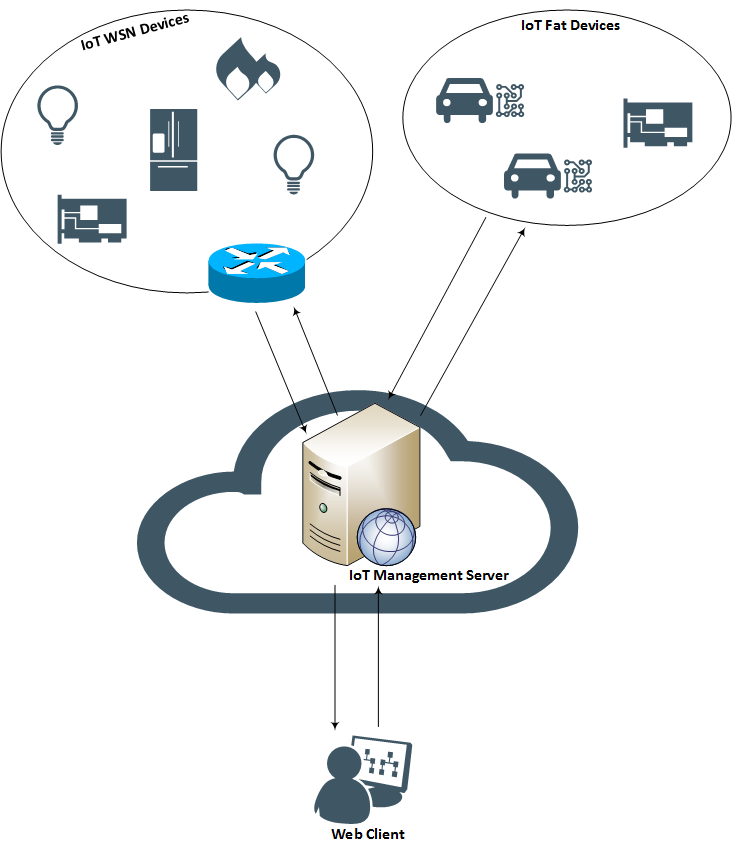
\includegraphics[scale=0.6]{images/systemuebersicht.png}
\caption{Systemübersicht}
\end{figure}
Der User kann seine IoT Devices entweder manuell erfassen, oder über ein Discovery ins System aufnehmen. Sobald ein Device im System ist, können hardware- und konfigurationsspezifische Parameter ausgelesen werden. Gemäss Use Case Analyse sind auch der Austausch von Dateien und das Absetzen von Kommandos vorgesehen.

Das Big Picture zeigt ein Deployment im Internet. Denkbar wäre sowohl die Bereitstellung mit einem eigenen Hosting, als auch in der Cloud bei einem Platform as a Service (PaaS) Anbieter. Benutzer der Management Applikation sollen über ein Web-GUI ihre IoT Devices administrieren können.
\newpage

\begin{landscape}
\section{Klassenstruktur}
\subsection{Klassendiagramm}
\begin{figure}[H]
\centering
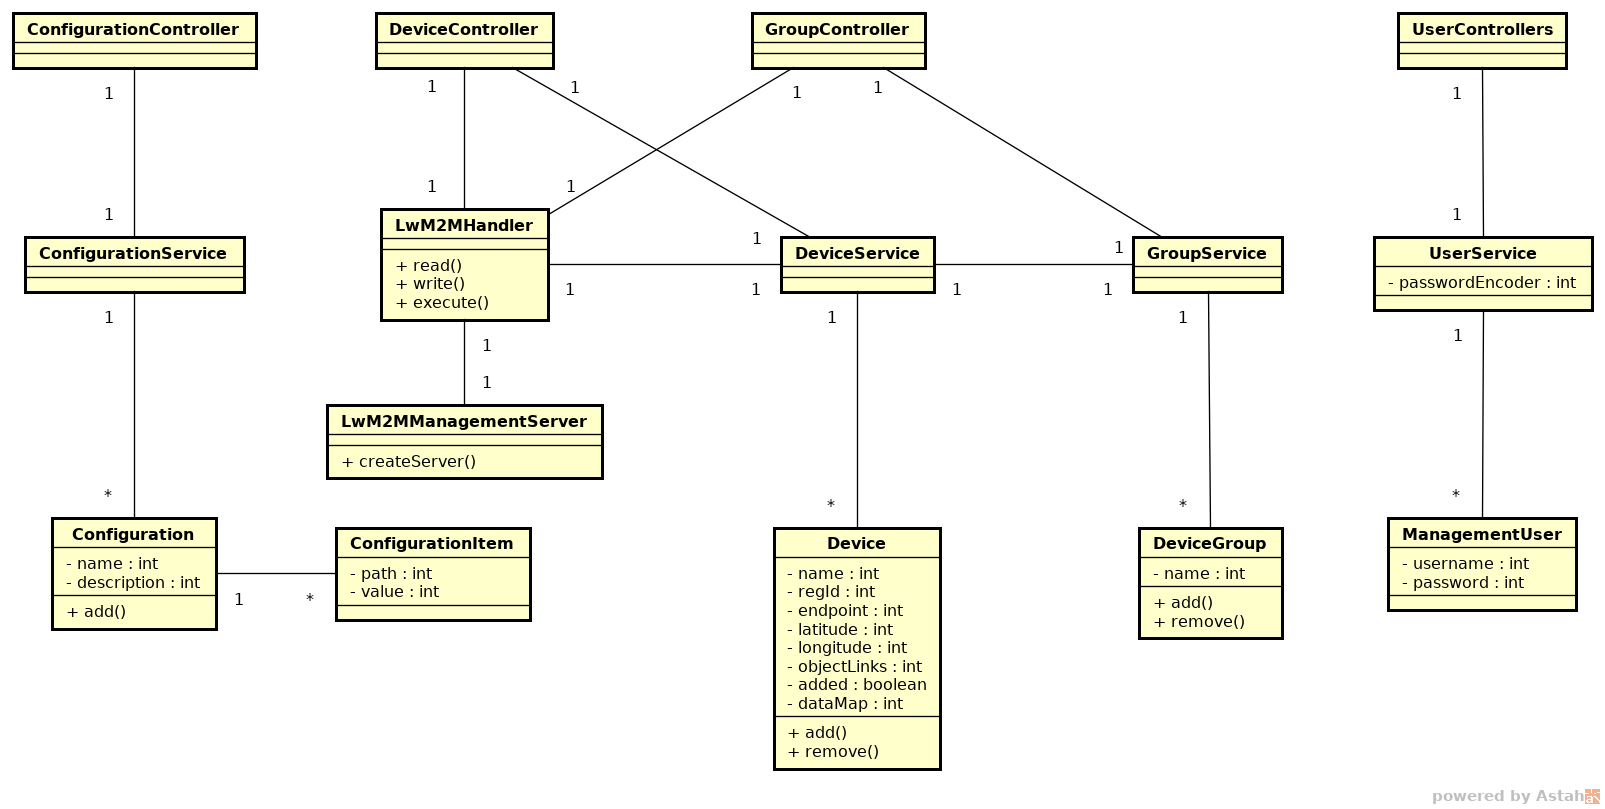
\includegraphics[width=1\textwidth]{images/domainmodel.png}
\caption{Klassendiagramm}
\end{figure}
\end{landscape}
\subsection{Klassenbeschreibungen}
\subsubsection{Connect}
Die Connect-Klasse ist für die Verbindung zu den Geräten zuständig. Sie behandelt die Authentisierung und stellt die Verbindung den anderen Klassen bereit. Dies ist eine zentrale Klassen, welche bei vielen Tätigkeiten benötigt wird.
\begin{table}[H]
\centering
    \begin{tabular}{@{}l p{14.1cm} @{}}\toprule    
    {Eigenschaft} & {Beschreibung}\\ \midrule
    connect() & Die Connect Methode, welche die Verbindung zu einem Device aufbaut.\\
    \bottomrule
    \end{tabular}
\end{table}

\subsubsection{Reader}
Mit dem Reader werden die Daten von den Devices abgefragt. Je nach Device wird eine andere Implementation der Read-Funktion bereitgestellt, damit alle gewünschten Protokolle unterstützt werden.
\noindent \begin{table}[H]
\centering
    \begin{tabular}{@{}l p{14.1cm} @{}}\toprule    
    {Eigenschaft} & {Beschreibung}\\ \midrule      
    read() & Read-Methode, welche die Daten vom gewünschten Device ausliest.\\
    \bottomrule
    \end{tabular}
\end{table}

\subsubsection{Writer}
Die Writer-Klasse schreibt die Kommandos und gewünschten Dateien zu einem Device. Diese Klasse wird für das Updaten, Konfig schreiben, so wie andere Parameter verwendet. Je nach Protokoll gibt es einen spezielle Implementation der Write-Klasse.
\noindent \begin{table}[H]
\centering
    \begin{tabular}{@{}l p{14.1cm} @{}}\toprule    
    {Eigenschaft} & {Beschreibung}\\ \midrule      
    write() & Die write-Methode schickt die gewünschten Daten zum Device. \\
    \bottomrule
    \end{tabular}
\end{table}


\subsubsection{Listener}
Dies ist die Discovery-Klasse. Mit der Listener-Klasse hören wir auf Geräte aus dem Netzwerk und falls welche Vorhanden sind, werden diese in der Datenbank eingefügt. Für die verschiedenen Protokolle gibt es verschiedene Implementationen
\begin{table}[H]
\centering
    \begin{tabular}{@{}l p{14.1cm} @{}}\toprule    
    {Eigenschaft} & {Beschreibung}\\ \midrule
    listen() &  Die Methode nach dem Starten über längere Zeit auf Device-Anfragen und speichert diese.\\
    \bottomrule
    \end{tabular}
\end{table}



\subsubsection{FileHandler}
Der FileHandler ist für den Up- und Download zuständig. Er nimmt alle Dateien entgegen und speichert diese auf dem Server ab. Oder er holt eine Datei vom Server und lädt diese herunter, damit man sie mit dem Writer auf ein Device schicken kann.
\begin{table}[H]
\centering
    \begin{tabular}{@{}l p{14.1cm} @{}}\toprule    
    {Eigenschaft} & {Beschreibung}\\ \midrule 
    upload() & Mit dem Upload wird eine Datei vom Filesystem auf das Managementtool geladen. \\
    download() & Durch den download, kann eine Datei vom Managementtool heruntergeladen werden. \\
    \bottomrule
    \end{tabular}
\end{table}

\subsubsection{Device}
Device ist eine Datenklasse, welche alle Angaben eines Devices speichert. Jedes Device wird so in ein Objekt gespeichert.
\begin{table}[H]
\centering
    \begin{tabular}{@{}l p{14.1cm} @{}}\toprule    
    {Eigenschaft} & {Beschreibung}\\ \midrule      
    name & Gerätenamen \\
    authType & Authentifikationstyp wie zum Beispiel Passwort oder Zertifikat  \\
    ipv4 &  IPv4-Adresse\\
    ipv6 &  IPv6-Adresse\\
    type &  Gerätetyp\\
    vendor & Gerätehersteller \\
    software & Software \\
	location &  Standortangaben des Devices\\    
    \bottomrule
    \end{tabular}
\end{table}

\subsubsection{DeviceGroup}
Durch die DeviceGroup-Klasse wird das Composite-Pattern umgesetzt. So können die Geräte individuell verschachtelt werden.
\begin{table}[H]
\centering
    \begin{tabular}{@{}l p{14.1cm} @{}}\toprule    
    {Eigenschaft} & {Beschreibung}\\ \midrule      
    name & Device Gruppen Namen\\
    description & Beschreibung der Device Gruppe \\
    \bottomrule
    \end{tabular}
\end{table}

\subsubsection{Credential}
Credential-Klasse für die Devices. Durch diese Datenklasse werden alle Usernamen/Passwort kombinationen gehashed abgespeichert. Zusätzlich werden auch die jeweiligen Zertifikate hinterlegt.
\begin{table}[H]
\centering
    \begin{tabular}{@{}l p{14.1cm} @{}}\toprule    
    {Eigenschaft} & {Beschreibung}\\ \midrule      
    username & Benutzername des Devices \\
    password & Devicepassword als Hash\\
    certificate & Zertifikat als Datenblob\\
    hash() & Hashmethode, damit die Passwörter nicht im Klartext gespeichert werden\\
    \bottomrule
    \end{tabular}
\end{table}

\subsubsection{Type}
Die Type-Klasse bestimmt die Verbindungsmethode, sowie das benutzte Protokoll. Diese werden pro Device erfasst.
\begin{table}[H]
\centering
    \begin{tabular}{@{}l p{14.1cm} @{}}\toprule    
    {Eigenschaft} & {Beschreibung}\\ \midrule      
    name & Name des Types \\
    connectionType & Typ der Verbindung, wie zum Beispiel Passwort oder Zertifikat\\
    protocoll & Verwendetes Verbindungsprotokoll\\
    \bottomrule
    \end{tabular}
\end{table}

\subsubsection{Command}
Mit der Command-Klasse werden alle benötigten Kommandos, wie zum Beispiel "Shutdown" usw. erfasst.
\begin{table}[H]
\centering
    \begin{tabular}{@{}l p{14.1cm} @{}}\toprule    
    {Eigenschaft} & {Beschreibung}\\ \midrule      
    command & Device-Kommando\\
    \bottomrule
    \end{tabular}
\end{table}


\subsubsection{File}
Das Interface File, bestimmt die Methoden und Variablen, welche die Vererbten Klassen implementieren müssen.
\begin{table}[H]
\centering
    \begin{tabular}{@{}l p{14.1cm} @{}}\toprule    
    {Eigenschaft} & {Beschreibung}\\ \midrule      
    name & Name der abgelegten Datei\\
    date & Datum\\ 
    Version & Versionsstand der Software oder der Konfigurationsdatei\\
    \bottomrule
    \end{tabular}
\end{table}


\subsubsection{ConfigFile}
Die ConfigFile-Klasse ist die Datenklasse für alle Konfigurationsdateien, damit diese in einer Datenbank angepassten Form gespeichert werden können. \begin{table}[H]
\centering
    \begin{tabular}{@{}l p{14.1cm} @{}}\toprule    
    {Eigenschaft} & {Beschreibung}\\ \midrule      
    - & -\\
    \bottomrule
    \end{tabular}
\end{table}



\subsubsection{SoftwareFile}
Diese Datenklasse ist das Objekt für eine Softwaredatei. So kann die Datei in der Datenbank erfasst werden.
\begin{table}[H]
\centering
    \begin{tabular}{@{}l p{14.1cm} @{}}\toprule    
    {Eigenschaft} & {Beschreibung}\\ \midrule      
    - & -\\
    \bottomrule
    \end{tabular}
\end{table}



\subsubsection{CertificateFile}
Zertifikatdatei-Datenklasse. Mit dieser Klasse werden Zertifikate in Objekte umgewandelt, damit man sie in der Datenbank abspeichern kann.
\begin{table}[H]
\centering
    \begin{tabular}{@{}l p{14.1cm} @{}}\toprule    
    {Eigenschaft} & {Beschreibung}\\ \midrule      
    - & -\\
    \bottomrule
    \end{tabular}
\end{table}


\section{Logische Architektur}
\begin{figure} [H]
	\begin{center}
	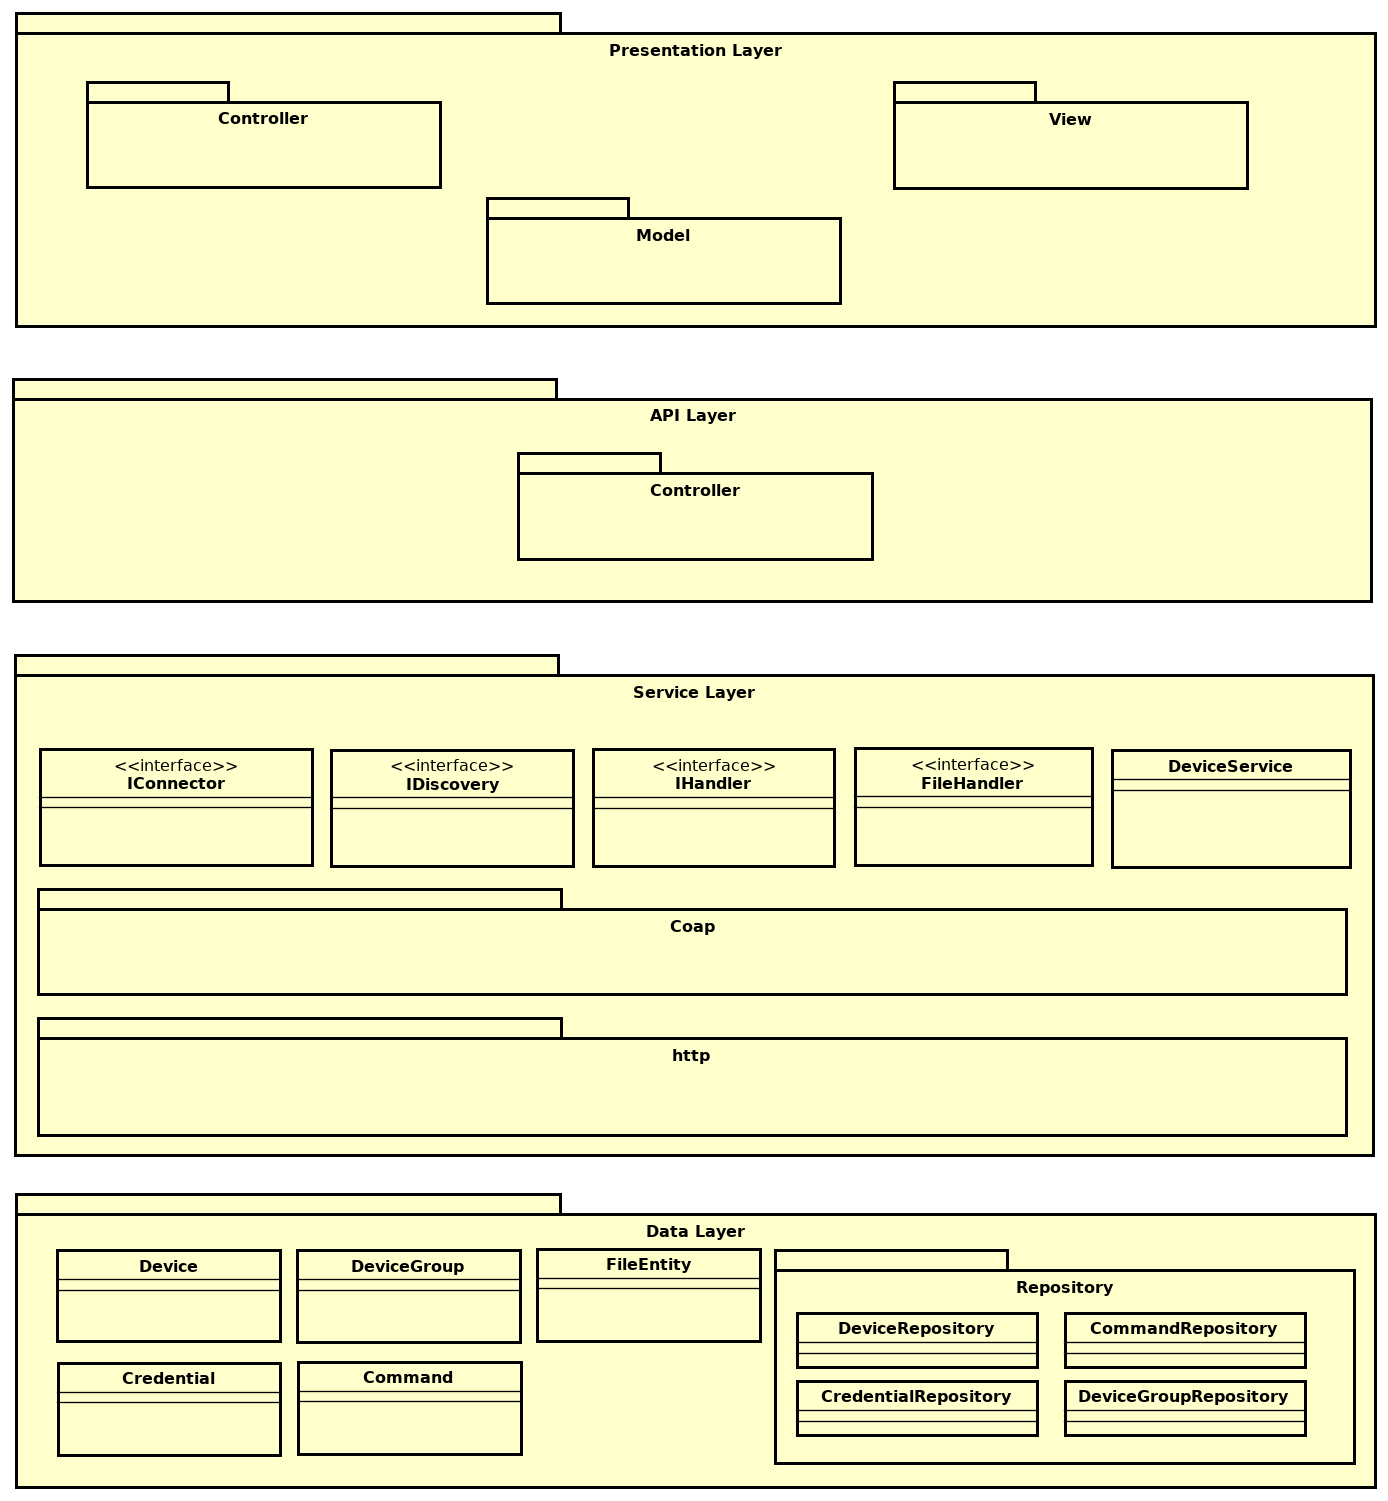
\includegraphics[width=0.90\textwidth]{images/architektur.png}
	\caption{Logische Architektur}
	\end{center}
\end{figure}


\subsection{Presentation-Layer}
Im Presentation-Layer wird das MVC-Pattern umsetzt. Dazu wird ein Controller, eine View sowie ein Model Package implementiert, welche alle Anfragen bearbeiten und anzeigen.
\subsubsection{Packagestruktur}
\begin{table}[H]
\centering
    \begin{tabular}{@{}l p{14.1cm} @{}}\toprule    
    {Packagename} & {Beschreibung}\\ \midrule
    Controller & Der Controller verwaltet alle Anfragen der View und bearbeitet das Model dementsprechend.\\       
    View & Die View bekommt von dem Model die Daten und Renderd dazu die jeweiligen Anzeigen. \\
    Model & Im Model werden alle Daten gehalten, welche die View anzeigt. Nur der Controller hat direkten Zugriff auf diese Daten. \\
    \bottomrule
    \end{tabular}
\end{table}
\subsubsection{Schnittstellen}
Der Presentation-Layer hat direkten Zugriff auf den Service-Layer. Bis jetzt besteht noch keine weitere Schnittstelle.


\subsection{Service-Layer}
Der Service-Layer beinhaltet alle Backend Klassen, welche für die Verarbeitung der Daten zuständig ist. Hier werden alle Devices erfasst, verbunden und verwaltet.
\subsubsection{Klassenstruktur}
\begin{table}[H]
\centering
    \begin{tabular}{@{}l p{14.1cm} @{}}\toprule    
    {Klassenname} & {Beschreibung}\\ \midrule
    Connect & Die Verbindungsklasse des Servicelayer stellt alle Verbindungen zu den Devices auf.  \\       
     Reader & Alle Daten von den jeweiligen Devices werden von der Reader-Klasse gelesen und an den Data-Layer weitergegeben.  \\       
     Writer &  Der Writer schreibt die gewünschten Daten auf ein Device und aktualisiert die Daten im Data-Layer \\       
     Listener &  Der Listener horcht auf neue Devices und erfasst diese laufend auf dem Data-Layer \\       
     FileHandler &  Mit dem FileHandler werden die Dateiobjekte auf dem Data-Layer erstellt und abgespeichert. \\       
    \bottomrule
    \end{tabular}
\end{table}
\subsubsection{Schnittstellen}
Der Service-Layer hat eine Schnittstelle zum Data-Layer. Durch den Service-Layer werden die Datenobjekte erstellt, bearbeitet und ausgewertet. Der Presentation-Layer muss immer über den Service-Layer, um eine saubere Abtrennung der Schichten zu gewährleisten.

\subsection{Data-Layer}
Der Data-Layer beinhaltet alle Datenobjekte, welche vom laufenden Programm benötigt werden. Diese werden von hier in die Datenbank geschrieben.
\subsubsection{Klassenstruktur}
\begin{table}[H]
\centering
    \begin{tabular}{@{}l p{14.1cm} @{}}\toprule    
    {Klassenname} & {Beschreibung}\\ \midrule
    Device & Device ist eine Datenklasse, welche alle Daten von einem Device beinhaltet.\\
    Credentials & Alle Zugriffsdaten der Devices sind in der Credentials-Klasse definiert. \\
    Type & Type beinhaltet die Typendefinition, welche den einzelnen Devices zugeordnet werden. \\
    DeviceGroup & In der Datenklasse DeviceGroup, werden alle Gruppen verwaltet, damit das Composite-Pattern umgesetzt werden kann.\\
    Command & Alle Kommandos werden zentral in der Command-Datenklasse gespeichert.\\
    FileEntitiy & In FileEntitiy wird das Grundgerüst für alle Dateien erstellt, damit diese in einer geeigneten Form in der Datenbank abgespeichert werden können.\\ 
    \bottomrule
    \end{tabular}
\end{table}
\subsubsection{Schnittstellen}
Der Data-Layer hat eine Schnittstelle zu der Datenbank.

\section{Architekturentscheidungen}
In diesem Kapitel werden alle Architekturentscheidungen aufgelistet, welche das Front-End, Back-End, sowie die Datenbank betreffen. Für jeden dieser Bereiche wurden Kriterien erarbeitet. Die Auswahl geschieht aufgrund der Bewertung anhand dieser Kriterien.

\subsection{Back-End}
Die Entscheidung des Frameworks für das Back-End ist von grosser Tragweite. Heutzutage existieren einige beliebte Frameworks um Web Applikationen zu erstellen. Die zu verwendende Programmiersprache ist bei vielen Frameworks ebenfalls unterschiedlich und sollte berücksichtigt werden.

\subsubsection{Kriterien}
\begin{itemize}
\item Open-Source Lizenz
\item Einfache Bedienung und schnelle Einarbeitung
\item Gute Dokumentation und Unterstützung durch die Community
\item Performance / Skalierbarkeit
\item Libraries für IoT Kommunikationsprotokolle
\item Kenntnisse der Programmiersprache
\end{itemize}

\begin{longtable}{| p{4cm} | p{11.7cm} |}
\hline
\textbf{Node.js}\newline

\includegraphics[width=0.25\columnwidth]{images/nodejs_logo.png} & Node.js ist eine Plattform für serverseitiges JavaScript. Das I/O-Handling ist event-driven und nicht-blockierend. Jeder Node.js Prozess ist single-threaded. Node.js hat viele Erweiterungsmodule wie z.B. Express um Web Applikationen zu erstellen. Für Web Applikationen ist Node.js mit Express besonders gut geeignet, da auf Client- und Serverseite mit JavaScript gearbeitet werden kann. Die Anzahl möglicher Verbindungen könnten trotz Single-Threading gut gehandled werden da die Anfragen asynchron mit einem Callback an die Devices gesendet werden, der aktive Thread würde somit nicht blockieren.
\newline
\newline
\textbf{Vorteile} \newline
\tabitem Einfacher Einstieg \newline
\tabitem Weite Verbreitung und gute Community-Unterstützung \newline
\tabitem Gute Skalierbarkeit (non-blocking) \newline
\tabitem Grundkenntnisse beim Entwicklerteam vorhanden \newline
\tabitem Gleiche Programmiersprache beim Front- und Backen \newline
\textbf{Nachteile} \newline
\tabitem Kein Multi-Threading \newline
\tabitem Interpretierte Skriptsprache \newline
\tabitem Schwache Objektorientierung (kein Polymorphismus, Duck-Typing, etc.)\\ \hline
\textbf{Spring MVC}\newline

\includegraphics[width=0.25\columnwidth]{images/spring_logo.png}
& Spring MVC wird verwendet um dynamische Webseiten mit Java Servlets zu erstellen. Dependency Injection und aspektorientierte Programmierung sind ebenfalls unterstützt. Konfigurationen über XML und Java Annotations unterstützen den Entwickler beim Erstellen von MVC Web-Applikationen. Die Library-Unterstützung für IoT spezifische Kommunikationsprotokolle wie beispielsweise CoAP sind bei Java EE hervorragend. Java unterstützt sowohl Multi-Threading, als auch non-blocking I/O. Gleichzeitige Verbindungen zu Devices könnten in eigene Threads ausgelagert werden, um nicht das gesamte Back-End zu blockieren.
\newline
\newline
\textbf{Vorteile} \newline
\tabitem Weite Verbreitung und gute Community-Unterstützung \newline
\tabitem Gute Skalierbarkeit (Multi-Threading) \newline
\tabitem Gute Java Programmierkenntnisse beim Entwicklerteam vorhanden \newline
\tabitem Kompilierte Sprache \newline
\tabitem Starke Objektorientierung (Polymorphismus, Type-Safety, etc.) \newline
\tabitem Dependency-Injection Unterstützung \newline
\textbf{Nachteile} \newline
\tabitem Umgang mit Spring MVC müsste vom Entwicklerteam erlernt werden \newline
\tabitem Unterschiedliche Sprachen für Front- und Back-End
\\ \hline 
\end{longtable}

\subsubsection{Skalierbarkeit}
Da potenziell viele Devices über die Applikation verwaltet werden könnten ist die Skalierbarkeit von grosser Bedeutung. Die Art der Verbindungen unterscheiden sich. Während die Anzahl gleichzeitiger Verbindungen über das Front-End zum Server (concurrent users) sehr gering sein wird, besteht die Möglichkeit, dass hunderte oder gar tausende IoT Devices verbunden sind.

Es besteht jedoch nicht die Notwendigkeit, dass während der Nutzungsdauer alle diese Verbindungen aufgebaut und offen gehalten werden. Es ist damit zu rechnen, dass niemals mehr als 100 gleichzeitige Verbindungen zu unterschiedlichen Devices existieren. 

\subsubsection{Entscheidung}
Die Entscheidung fiel auf Spring MVC. Eine Implementation mittels Node.js und Express wäre ebenfalls denkbar, da alle Anforderungen und Restriktionen erfüllt werden könnten. Auch andere Frameworks wie Django oder Ruby on Rails würden ebenfalls in Frage kommen, wurden aber nicht berücksichtigt da keine oder nur kaum Vorkenntnisse beim Entwicklerteam vorhanden waren.

Ausschlaggebend für die Auswahl von Spring MVC ist die zugrundeliegende Programmiersprache Java. Die Unterstützung von Klassen, Vererbung und Polymorphie sowie die grosse Unterstützung von Tools und Plugins ermöglichen eine angenehmere und übersichtlichere Entwicklung. Durch die Unterstützung mittels XML Konfigurationen und Java Annotations werden die Entwickler mit Spring MVC hervorragend unterstützt.

\newpage
\subsection{Front-End}
Das Front-End der Applikation muss dem Benutzer auf eine einfache und übersichtliche Weise die Interaktion ermöglichen. Es sollen einerseits neue Geräte hinzugefügt werden, andererseits bestehende Geräte verwaltet oder überwacht werden. Potenziell könnten eine grosse Anzahl solcher IoT Devices vorliegen, weshalb diese übersichtlich gruppiert werden sollen.

\subsubsection{Kriterien}
\begin{itemize}
\item Webbasierter Zugriff
\item Responsive Web Design für unterschiedliche Bildschirmgrössen
\item Open-Source Lizenz
\item Einfache Bedienung und schnelle Einarbeitung
\item Gute Dokumentation und Unterstützung durch die Community
\end{itemize}

\subsubsection{Varianten}
Bei der Variantenauswahl wurden drei sich stark unterscheidende Ansätze gewählt. Grundsätzlich wären weitere Frameworkalternativen zu Bootstrap und Angular.js denkbar.

\begin{longtable}{| p{4cm} | p{11.7cm} |}
 \hline
  \textbf{Hardcoding} & Hardcoding des Frontends bringt wenige Vorteile. Sämtlicher HTML, CSS und JavaScript Code müsste von Hand geschrieben werden. Ein selber erstelltes responsives Layout mit CSS ist zwar möglich, aber aufwändig. Es müsste somit viel Zeit in das Layout und das Styling für ein ansprechendes Ergebnis investiert werden. Eine Cross-Browser Unterstützung ist ebenfalls schwierig.\\ \hline 
 \textbf{Twitter Bootstrap} & Bootstrap von Twitter ist ein weit verbreitetes Framework für Webseiten. Responsive Layouts für unterschiedliche Bildschirmgrössen werden unterstützt. Elemente wie Buttons, Drop-Down Menüs und ähnliches werden von Bootstrap auf sehr einfache Weise bereitgestellt. Die JavaScript Funktionalitäten beschränken sich auf die Anzeige von UI Elementen. Falls JavaScript für die Programmierung der Applikation verwendet wird sollte ein weiteres Framework dafür verwendet werden.\\ \hline 
 \textbf{Angular.js} & Angular.js ist ein bekanntes Framework für Single Page Applications (SPA) im MVC Stil. Angular.js ist TypeScript 2 basiert, hat Dependency Injection Mechanismen eingebaut, unterstützt 2-way Databinding und Unit Testing. Die Software Architektur ist Client-konzentriert, MVC passiert im Browser.\\ \hline
\end{longtable}

\subsubsection{Entscheidung}
Durch die einfache und schnelle Entwicklungsmöglichkeiten wurde Bootstrap gewählt. Angular.js hat klare Vorteile bei der Erstellung von Single Page Applications. Nach jetztigen Erkenntnissen sind jedoch keine aufwändigen Funktionen clientseitig vorgesehen, Data-Binding scheint zum heutigen Zeitpunkt nicht notwendig. 

Dem Projektteam ist Angular.js unbekannt und es müsste mit einer langen Einarbeitungszeit und anfänglich schlechter Code-Qualität gerechnet werden. Falls zu einem späteren Zeitpunkt weitere Anforderungen und Funktionen vorgesehen werden, wäre eine \glqq echte\grqq  Single Page Application mit Angular.js eine echte Alternative und könnte die \glqq einfache\grqq  Variante mit Bootstrap von Twitter ergänzen oder ablösen.

\newpage
\subsection{Datenbanktechnologie}
Für die Persistierung der Objekte stehen zwei grundlegende Verfahren zur Verfügung. SQL (Structured Query Language) war über einen langen Zeitraum die Standardtechnologie für die Persistierung von Datenobjekten, mit NoSQL Technologien ist jedoch eine starke Alternative mit einigen Vorteilen gegenüber der herkömmlichen SQL Technologie entstanden.

\subsubsection{SQL}
SQL basiert auf einem relationalen Datenmodell. Die Objeke werden auf Tabellen abgebildet. Eine Tabelle stellt somit ein Typ- und die Columns Felder dar. Mit SQL-Datenbanken wird ein stark normalisiertes Datenmodell ohne Redundanzen angestrebt. Mittels referenzieller Integrität (Fremdschlüsselwerte in Tabelle X müssen als Primärschlüsselwerte in Tabelle Y vorhanden sein) wird eine starke Datenkonsistenz gewährleistet. Ein Datensatz kann daher nur gelöscht werden, wenn keine Referenzen darauf zeigen. Mittels Joins von Tabellen können zusammenhängende Datensätze mit einem einzelnen Query abgefragt werden.

Ein grosser Nachteil bei SQL ist das strikte Datenschema. Die Tabelle gibt genau vor, welche Columns für das Objekt existieren (müssen). Möchte man weitere Werte respektive Columns hinzufügen, so müsste das gesamte Schema der Tabelle angepasst werden (altering).

\subsubsection{NoSQL}
Mit NoSQL werden die Daten als Key-Value Paare in einem strukturierten Format gespeichert. Häufig ist dies JSON (JavaScript Object Notation). Eine Collection steht für einen Typ von Daten und enthält entweder Key-Value Paare oder weitere Collections. Beziehungen zu anderen Objekten können auf zwei verschiedene Arten erfolgen; entweder als embedded Collection (Denormalisierung) oder mittels Referenz auf ein anderes Objekt.

Ein grosser Vorteil ist das flexible Datenmodell. Wenn man sich beispielsweise ein persistiertes Device-Objekt anschaut, so könnte dies wie folgt aussehen:
\begin{lstlisting}[language=json]
{
    "_id":{
        "id": "58ecfe09beedc31188fc0281",
        "name":  "Device XY",
        "protocolType": "HTTP",
        "authType": "BASIC_AUTH",
        "endpoint": "http://some.domain.com/path",
        "username": "admin",
        "password": "1234"
        }    
}
\end{lstlisting}
Falls ein weiteres Attribut gespeichert werden müsste, ist dies bei NoSQL nicht weiter problematisch. Die Datenbank speichert die Objekte auch mit anderen Attributen resp. Key-Value Paaren.

\newpage
NoSQL selbst unterteilt sich in verschiedene Datenmodelle. \cite{WikiNoSQL}
\begin{longtable}{| p{4cm} | p{11.7cm} |}
\hline
\textbf{Key-Value} & Leistung: hoch \newline Skalierbarkeit: hoch \newline Flexibilität: hoch \newline Komplexität: keine \newline Funktionalität: keine \newline
Durch die Einfachheit des zugrunde liegenden Datenmodells lassen sich Datensätze schnell (in O(1)) abfragen. Komplexere Abfragen über Verknüpfung der Objekte sind deutlich langsamer. Bei einer hohen Frequenz von Abfragen und Speicherung von Key-Value Tupeln ist diese Form von Datenbank geeignet.
\\ \hline
\textbf{Spaltenorientiert} & Leistung: hoch \newline Skalierbarkeit: hoch \newline Flexibilität: mittel \newline Komplexität: gering \newline Funktionalität: minimal \newline
Das zugrunde liegende Datenmodell basiert auf der Speicherung der Spaltenwerte. Während normalerweise Datensätze auf einer Zeile mit ihren unterschiedlichen Spalten abgelegt werden, so wird bei dieser Art zuerst eine komplette Spalte gespeichert bevor mit Werten aus einer anderen Spalte forgefahren wird. 
\\ \hline
\textbf{Dokumentenorientiert} & Leistung: hoch \newline Skalierbarkeit: hoch \newline Flexibilität: hoch \newline Komplexität: gering \newline Funktionalität: gering \newline
Dokumente bilden das Schema einer Entität. Eine dokumentenbasierte Datenbank kann mehrere solcher Dokumente enthalten. Dokumente sind quasi das Gegenstück zu Tabellen in einer relationalen Datenbank. Ein Dokument liegt meist im JSON Format vor und hält seine Objekte eingebettet. 
\\ \hline
\textbf{Graphbasiert} & Leistung: unterschiedlich \newline Skalierbarkeit: unterschiedlich \newline Flexibilität: hoch \newline Komplexität: hoch \newline Funktionalität: gem. Graphentheorie \newline
Eine Graphendatenbank speichert Knoten und Kanten. Knoten sind Entitäten und Kanten deren Beziehungen. Dieses Datenmodell eignet sich für die Modellierung und Speicherung von Netzwerken wie beispielsweise Social Media.
\\ \hline
\end{longtable}

\subsubsection{Entscheidung}
NoSQL wurde als geeignetere Variante für die Speicherung der Objekte ausgewählt. Bei vielen unterschiedlichen Devicetypen muss davon ausgegangen werden, dass Änderungen respektive Ungleichheiten am Schema auftauchen werden. Ein starres, relationales Modell würde dies stark erschweren, da jedesmal mittels \glqq ALTER TABLE\grqq  das Schema geändert- und bestehende Datensätze angepasst werden müssten.

Als NoSQL Implementation wurde \glqq mongoDB\grqq ausgewählt. MongoDB ist eine dokumentenorientierte Datenbank, welche Objekte im BSON Format abspeichert. Die Entitäten werden in sogenannten \glqq Collections\grqq  abgelegt. Attribute der Collections können einzeln abgefragt werden. Die Struktur der Collections ist flexibel, Attribute von Objekten innerhalb der Collections dürfen sich unterscheiden. MongoDB ist die zurzeit wohl am weitest verbreitete NoSQL Implementation, weshalb eine grosse Community und umfangreiche Online-Hilfen verfügbar sind.
 




